% Author: Pavol Loffay
% Project: Master thesis - Hawkular alert prediction
% Date 20.2.2015

% Cross-Referencing Conventions:
% chap: chapter
% sec: section
%
% appen: everything from appendix, e.g. appen:img:foo
%
% eq: equation
% img: image
% tab: table
% alg: algorithms
% item: item in itemize
%
% example \label{img:foo-foo}
%%%%%%%%%%%%%%%%%%%%%%%%%%%%%%%%%%%%%%%%%%%%%%%%%%%%%%%%%%%%%%%%%%%
\chapter{Introduction} \label{chap:introduction}
When driving successful business on the internet, it is important to assure application`s health and reliability. One
can achieve that by monitoring subjected resources and setting up clever alerting system.

These features are offered by many monitoring systems, however being predictive in this area can even prevent
undesirable states and most importantly gives administrators more time to react to such \\events. For instance it
can decrease downtime of an application or ability to load balance workload in advance by horizontal scaling of
targeted services.

Alerting systems are sophisticated and can be composed by many conditions. This work focuses on predicting future
metric values \\which are then sent as input for evaluation to alerting system.

The work starts with time series theory by describing various approaches for time series modelling and forecasting.
The chapter describes models which are used within the work, could be used or explains why the decision was made to
use other models.

Following chapter demonstrates models from previous chapter on real time series. It visually shows predictive
capabilities of targeted models and compares produced statistical quantities.

The third chapter briefly describes existing monitoring and management solutions which are to some extend
Hawkular competitors. Java libraries for time series forecasting are also mentioned there.

The fourth chapter describes implementation part of the thesis. It starts with core artifacts for time series
forecasting and continues to building web application and integration into Hawkular.

The last chapter is dedicated to the evaluation of the forecasting accuracy of the implemented solution.
Models from \texttt{forecast} package from language R were chosen as a referential implementation.

    %%%%%%%%
    \section{Hawkular} \label{sec:hawkular}
    The implementation part of the master's thesis is developed as a part of an open source project
    Hawkular\footnote{Available at \url{http://www.hawkular.org}}, therefore, the application architecture and used
    technologies had to fit into the overall project design.

    Hawkular is middleware monitoring and management platform developed by company Red Hat and independent community
    of contributors. It is a successor of very successful RHQ\footnote{Available at
    \url{https://rhq-project.github.io/rhq/}.} project, also known as JBoss Operations Network (JON). By monitoring,
    it is meant that there are agents for diverse applications which push data to the server. These agents can also
    execute application specific actions.

    The monolithic architecture of the RHQ project was due to its size hard to maintain and lacking robust REST API
    lead to fresh development of new application. Hawkular, in contrast, consists of several loosely coupled or even
    independent applications. These independent components are much easier to maintain and what is more important they
    communicate over REST API.

    This architecture of microservices and chosen protocol allow simple development of agents which can be
    written in any programming language. In RHQ only Java agent were available.

    Hawkular as a product itself is customized
    Wildfly\footnote{An open source project of JBoss Enterprise Application Platform.} application server with all
    components deployed in it.

    List of Hawkular main components:
    \begin{itemize}
        \item Console\,--\,user web interface.
        \item Accounts\,--\,authorization subsystem based on Keycloak\footnote{An open
            source single sing-on and identity management for RESTful web services.}.
        \item Inventory\,--\,graph based registry of all entities in Hawkular.
        \item Metrics\,--\,time series metrics engine based on Cassandra\footnote{An open
            source distributed database management system. Hybrid between key-value and
        column-oriented database.}.
        \item Alerts\,--\,alerting subsystem based on JBoss Drools.
    \end{itemize}

    Some of the modules also use Java messaging system (JMS) for inter-component communication.

    Modules are packaged as standard Java web archives (WAR), or enterprise archives (EAR) and deployed into Wildfly.
    Build and package management is performed by Maven and Gulp for user interface modules.

    %%%%%%%%
    \section{Data Mining Goals} \label{sec:goals}
    The goal of this thesis is to develop a module for Hawkular which will provide forecasts for any time series
    metrics collected by agent.

    Module should learn from new incoming metric data and immediately send predicted values for future timestamps to
    alerting subsystem. Based on this values an alert can be triggered. This implies that forecasting engine should
    work on continuous flow of data. Forecast should be also available for user interface in predictive charts.

    One Wildfly agent on average collects hundreds to thousands metrics, therefore module should be capable of
    processing high volume of data. Some of the customers monitor hundreds of servers, each with multiple agents.
    Therefore performance of chosen learning algorithm has to be taken in the account.

    %%%%%%%%
    \section{Metrics in Hawkular} \label{sec:metrics-in-hawkular}
    In Hawkular, there are three types of metrics: gauge, counter and availability. All of them are univariate metrics
    of structure \\$\{timestamp, value\}$. Each of these types is used for collecting dedicated types of metric data.
    For example gauge can increase or decrease over the time, counter monotonically decreases or increases and
    availability represents up or down state of a resource.

%%%%%%%%%%%%%%%%%%%%%%%%%%%%%%%%%%%%%%%%%%%%%%%%%%%%%%%%%%%%%%%%%%%
\chapter{Time Series Models} \label{chap:models}
This chapter focuses on time series theory and various approaches for time series modelling. Models are put in
order from simpler to more complex ones. Only some of the discussed models are selected for the implementation.
Chapter also adds some theory necessary for time series analysis, for example unit root tests,
seasonal decomposition and period identification of seasonal time series.

From the goals from Section \ref{sec:goals} results that selected time series models should be robust enough to work on
arbitrary monitored time series and at the same time to be computationally inexpensive when it comes to learning and
forecasting process.

Firstly, it is important to define time series; it is a sequence of observations $s_t \in \mathbb{R}$ put in order of
time. This thesis focuses only on univariate equidistant discrete time series.

Time series analysis contains many segments, this work aims on forecasting only. It is defined as a process of making
prediction of the future based on the past. In other words, forecasting is possible because future depends on the
past or analogously because there is a relationship between the future and the past. However, this relation is not
deterministic and can be hardly written in an analytical form \cite{otexts}.

Generally there are two forecasting types: qualitative and quantitative. Qualitative methods are mainly based on the
opinion of the subject and are used when past data are not available, hence not suitable for this project. If there
are past data available, quantitative forecasting methods are more suitable.

    %%%%%%%%
    \section{Simple Quantitative Models} \label{sec:simple-models}
    Following methods are the simplest forecasting quantitative models. They can be used for any time series without
    any prerequisites or further analysis.

    \begin{itemize}
        \item Average method\,--\,forecasts are equal to the value of the mean of historical data.
            \begin{eqnarray}
                \hat{y}_{T+h|T} = \overline{y} = (y_{1}+ \dots + y_{T}) / T 
            \end{eqnarray}
        \item Na\"{i}ve method\,--\,forecasts are equal to the last observed value.
            \begin{eqnarray}
                \hat{y}_{T+h|T} = y_{T}
            \end{eqnarray}
        \item Drift method\,--\,variation of na\"{i}ve method which allow the forecasts to increase or decrease
            over time.
            \begin{eqnarray}
                \hat{y}_{T+h|T} = y_{T} + \frac{h}{T-1} \sum_{t=2}^T{y_{t} - y_{t-1}} = 
                    y_{T} + h(\frac{y_{T}-y_{1}}{T-1}) 
            \end{eqnarray}
    \end{itemize}

    There are also seasonal variants of these models which hold one model for each season. These methods in general
    produces high forecasting error but are very easy to implement.

    %%%%%%%%
    \section{Linear Regression} \label{sec:linear-regression}
    Linear regression is a classical statistical analysis technique. It is mostly used to determine whether there is
    linear relationship between dependent and eventually more independent variables \cite{cipra}. It is also used for
    predictions mainly in econometric field.

    Simple linear regression is defined as:

    \begin{eqnarray} \label{eq:linear-regression}
        y = \beta_0 + \beta_1 x + \epsilon
    \end{eqnarray}

    Parameters $\beta_0$ and $\beta_1$ are calculated by minimizing the sum of squared errors:
    
    \begin{eqnarray} \label{eq:linear-regression-estimation}
        SSE = \sum_{i=1}^N \epsilon_{i}^2 = \sum_{i=1}^N (y_i - \beta_0 - \beta_1 x_i)^2
    \end{eqnarray}
    
    Once the parameters are estimated, predictions for any time in the future can be calculated. If modelled time
    series is not stationary and trend changes over time parameters should be periodically reestimated to achieve
    better forecasting accuracy. This means the regression model does not adapt if the underlying time series changes.

    %For econometric analysis it is important to use best linear unbiased estimator,
    %where couple of assumptions has to hold:
    %\begin{enumerate}
    %    \item $E(Y_i) = \beta_0 + \beta_1 X_i$
    %    \item $var(Y_i)=\sigma^2$\,--\,homoscedasticity
    %    \item $cov(Y_i, Y_j)=0$, for $i \neq j$
    %    \item $Y_i$ cames from normal distribution
    %    \item $X_i$ is not random variable
    %\end{enumerate}
    %Where $i$ takes values from $1$ to the number of observed values. These assumptions 

    %%%%%%%%
    \section{Simple Exponential Smoothing} \label{sec:simple-ex}
    The concept behind simple exponential smoothing is to attach larger weights to the most recent observations than
    to the observations from distant past. Forecasts are calculated using weighted averages where the weights
    decrease exponentially as observations come from further in the past \cite{hyndman-state-space}. In other words,
    smaller weights are associated with older observations. Equation for simple exponential smoothing is listed in
    \ref{eq:simple-ex}.

    \begin{gather} \label{eq:simple-ex}
         \hat{y}_{T+1|T} = l_t \\ \nonumber
         l_t = \alpha y_t + (1-\alpha)l_{t-1}
    \end{gather}

    For smoothing parameter $\alpha$ holds $ 0 \leq \alpha \leq 1 $. Note, if $\alpha = 1$ then \\
    $\hat{y}_{T+1|T} = y_{T}$ so forecasts are equal to the na\"{i}ve method. If the parameter $\alpha $ is smaller
    more weight is given to the observations from distance in the past.

    Simple exponential smoothing has a flat forecast function, that means all forecasts are the same.
    Therefore this method is useful if a series does not contain any trend or one is interested only in one step
    ahead prediction. Multi step ahead predictions for time series with trend usually produce high error rate.

    This model is generally used for noise separation or trend estimation.

    %%%%%%%%
    \section{Holt's Liner Trend Model} \label{sec:double-ex}
    Simple exponential smoothing can be extended to allow forecasting of data with a trend. This was done by
    Charles C. Holt in 1957. This method is slightly more complicated than the original one without trend.
    In order to add trend component another equation has to be added \ref{eq:holt}.

    \begin{gather} \label{eq:holt}
        \hat{y}_{t+h|t} = l_{t} + hb_{t} \\ \nonumber
         l_t = \alpha y_t + (1 - \alpha) (l_{t-1} + b_{t-1}) \\ \nonumber
         b_t = \beta (l_t - l_{t-1}) + (1 - \beta)b_{t-1} 
    \end{gather}

    Parameter $b_t$ denotes a slope of the series and the parameter $l_t$ level. There is also a new smoothing
    parameter for the slope\,--\,$\beta$. Its rage is equal to $\alpha$, so $\alpha,\beta \in \interval[{0,1}]$.

    %%%%%%%%
    \section{Holt-Winters Seasonal Model} \label{sec:triple-ex}
    This model is an extension of Holt's linear trend method with added seasonality. It is also called triple
    exponential smoothing. There are three equations in this model \ref{eq:holt-winters}. One for level, second for
    trend and third for seasonality. Each pattern uses smoothing constant $ \alpha,\beta,\gamma \in \interval[{0,1}]$.

    \begin{gather} \label{eq:holt-winters}
        \hat{y}_{t+h|t} = l_{t} + hb_{t} + s_{t+h_m-m}\\ \nonumber
        l_t = \alpha (y_t - s_{t-m}) + (1 - \alpha) (l_{t-1} + b_{t-1}) \\ \nonumber
        b_t = \beta (l_t - l_{t-1}) + (1 - \beta)b_{t-1} \\ \nonumber
        s_t = \gamma (y_t - l_{t-1} - b_{t-1}) + (1-\gamma)s_{t-m}
    \end{gather}

    Where $h_m=[(h-1) \mod m] + 1$, which ensures that the estimates of the seasonal indices came from the correct
    season. This model can be used only if the period of time series is know beforehand. In Hawkular the period  of
    the time series is unknown, therefore period identification should be also implemented.

    Each exponential smoothing model contains parameters which should be precisely estimated ($\alpha, \beta,
    \gamma$), but it is also possible to use default values from literature. However, with default values models produce
    higher forecasting error than with estimated parameters. Estimation process defines objective function which
    value can be mean squared error, mean absolute error or likelihood. Then this objective function is passed to
    non-linear optimization algorithm.

    Time complexity of exponential smoothing models for learning $N$ observations is $O(N)$. With enabled optimization
    the complexity depends on used optimization algorithm.

    Exponential smoothing models have advantage over other more complicated models that if a system needs to achieve high
    performance than default parameters can be used. This would not be possible with ARIMA models for instance.

    %%%%%%%%
    \section{Box\,--\,Jenkins Methodology (ARIMA)} \label{sec:arima}
    Models from Box\,--\,Jenkins methodology are the most widely used in time series analysis for econometric data.
    This methodology is based on analysis of autocorrelation (ACF) and partial autocorrelation \\(PACF) functions.
    
    The most generic model is ARIMA(p, d, q). It combines autoregressive, integrated and moving average parts together.
    An autoregressive model (AR) consist of sum of weighed lagged observations \ref{eq:ar-model}.
    The order of this model is defined by $p$ and can be determined from PACF function \cite{cipra}.

    \begin{gather} \label{eq:ar-model}
        y_t = \phi_1 y_{t-1} + \phi_2 y_{t-2} + \dots + \phi_p y_{t-p} + \epsilon_t \\ \nonumber
        \epsilon_t \overset{iid}{\sim} N(0, \sigma^2)
    \end{gather}

    A moving average model (MA) is a sum of weighted errors of order $q$. The order of this part can be determined
    from ACF function \cite{cipra}. Moving averages model should not be confused with simple moving average from
    \ref{sec:simple-ex} which is used for trend estimation. In moving average model MA(q) the current value is a
    regression against white noise of prior values of the series \cite{wiki-ma-model}. A random noise from each
    point is assumed to come from the same distribution which typically is a normal distribution.  Model of the order
    $q$ is listed in \ref{eq:ma-model}.

    \begin{gather} \label{eq:ma-model}
        y_t = \theta_1 \epsilon_{t-1} + \theta_2 \epsilon_{t-2} + \dots + \theta_p y_{t-q} + \epsilon_t \\ \nonumber
        \epsilon_t \overset{iid}{\sim} N(0, \sigma^2)
    \end{gather}

    The last part of the model is used when a time series is non stationary. There are several ways how to make a
    particular time series stationary. Box\,--\,Jenkins methodology uses differencing\,--\,integration part I(d).  The
    order of differentiated original series is denoted by $d$ letter. Usually first order differences are enough to
    make a time series stationary.

    It is important to mention that models AR(p) and MA(q) are invertible. Therefore any stationary AR(p) model can
    be written as \\MA($\infty$) and with some assumptions vice versa \cite{brockwell}. ARIMA model is often written
    with backshift operator $By_t=y_{t-1}$. With this operator \\ARIMA(p, d, q) is listed in \ref{eq:arima}. On the
    left side of the equation is AR(P) process and on the right MA(q).

    \begin{gather} \label{eq:arima}
        (1- \phi_1B - \dots - \phi_pB^p)(1-B)^d y_t = \\ \nonumber
         c + (1+\theta_1B+\dots+\theta_qB^q) \epsilon_t
    \end{gather}

    The parameters of the model, including AR and MA part can by estimated by non-linear optimization algorithm
    with likelihood as objective function \cite{brockwell}. However this function is much more complicated than for
    exponential smoothing models. For successful estimation a certain number of historical points needs to
    be available. Reference \cite{cipra} advises minimal training size of at least fifty observations.

    After this theoretical part it is clear that ARIMA models are more complicated than family of moving averages.
    To this also refers \cite{hyndman-forecasting} and adds that ARIMA models are less robust than exponential
    smoothing models.

    %%%%%%%%
    \section{Artificial Neural Networks} \label{sec:ann}
    Recently a large number of successful applications using neural networks for time series modeling show that they
    can produce valuable results \cite{ann-forecasting-state-art}. There are several non trivial issues with
    determining the appropriate architecture of the network. This has to be taken into account because it can
    dramatically effect learning performance and forecasting accuracy \cite{ann-model-selecting}.
    Besides the problems with selecting right architecture learning process of artificial neural network is much more
    computationally expensive than selecting appropriate ARIMA or exponential smoothing model \cite{ann-forecasting}.

    Because Hawkular forecasting engine should be capable of predicting thousands of metrics at the same time, models
    based on neural networks would have too high computational requirements, therefore, they are not suitable for our
    environment.

    %%%%%%%%
    \section{Time Series Decomposition} \label{sec:decomposition}
    In modelling time series it is sometimes necessary to decompose series to trend, seasonal and random component
    \cite{otexts}. It is also used for initialization seasonal indices in triple exponential smoothing.

    \begin{itemize}
        \item \textbf{Trend $ T_{t} $}\,--\,exists if there is long term increase or decrease over
            time. Can be linear or nonlinear (e.g. exponential growth).
        \item \textbf{Seasonal $ S_{t} $}\,--\,exists when a series is influenced by seasonal factors.
            Seasonality is always of fixed and known period.
        \item \textbf{Cyclic $ C_{t} $}\,--\,exists if there are long term wave-like patterns.
            Waves are not of a fixed period.
        \item \textbf{Irregular $ E_{t} $}\,--\,unpredictable random value referred as white
            noise. 
    \end{itemize}

    Decomposition can be written in many forms. Two of them are additive \ref{eq:decom-additive} and multiplicative
    \ref{eq:decom-multi}. Which one to use depends on the underlying time series model.

    \begin{gather} \label{eq:decom-additive}
        y_{t} = T_{t} + S_{t} + C_{t} + E_{t} \\
        y_{t} = T_{t} \times S_{t} \times C_{t} \times E_{t} \label{eq:decom-multi}
    \end{gather}

    An algorithm for additive decomposition consists of following steps:

    \begin{enumerate}
        \item Compute a trend component $\hat{T}_t$ using moving average model. If a period is even use
        $2 x MA(period)$. If period is an odd use $MA(period)$. $2 x MA$ for even period is used because it
        has to be symmetric.
        \item Calculate detrended series $y_t - \hat{T}_t$.
        \item Estimate seasonal indices $\hat{S}_t$ for each period by averaging values of given period. For example,
         the seasonal index for Monday is the average for all detrended Monday values in the data. Then the mean of
         seasonal indices is subtracted from each period.
        \item Random component is calculated by subtracting trend and seasonal component from original time series
            $\hat{E}_t = y_t - \hat{T}_t - \hat{S}_t$.
    \end{enumerate}

    %%%%%%%%
    \section{Augmented Dickey\,--\,Fuller Test} \label{sec:adf}
    Time series statistical tests are often used for testing if there is particular characteristics present in time
    series. Unit root tests are used whether a time series is stationary. In this work Augmented \\Dickey\,--\,Fuller
    (ADF) test was chosen for unit root testing.

    Its null hypothesis is \emph{$H_0$: time series contains a unit root}\,--\,it is not stationary. Outcome of this
    test
    is a negative ADF statistics. The more negative it is the stronger the rejection of the hypothesis.
    The full form of ADF test is listen in \ref{eq:adf-test}.

    \begin{gather} \label{eq:adf-test}
        \Delta y_t = \alpha + \beta t + \gamma \Delta y_{t-1} + \dots + \delta{p-1} \Delta y_{t-p+1} + \epsilon_t \\
        ADF = \frac{\hat{\gamma}}{SE(\hat{\gamma})} \label{eq:adf-stat}
    \end{gather}

    There are multiple variants of ADF test. Some of them leave out parts of equation \ref{eq:adf-test}. The most
    important ones and widely used are:

    \begin{itemize}
        \item \emph{nc}\,--\,for regression with no constant nor time trend ($\beta t$)
        \item \emph{c}\,--\,for regression with an intercept but no time trend ($\beta t$)
        \item \emph{ct}\,--\,for regression with an intercept and time trend
    \end{itemize}

    Each of them is good when testing particular type of stationarity. For example for testing if there is trend
    present in the time series \emph{c} version is the best choice.

    The implementation of this test fits multiple linear regression model from equation \ref{eq:adf-test} and
    calculates ADF statistics listed in \ref{eq:adf-stat}. SE denotes standard error of estimated $\hat{\gamma}$.

    %%%%%%%%
    \section{Seasonality Detection} \label{sec:period-detection}
    Forecasting engine in Hawkular system does not have any inside information about period of a time series being
    modelled, therefore, automatic period identification has to be implemented. In practice it is a difficult task and
    result often differs from correct period, especially if there is significant noise present in the series
    \cite{period-meteo}.

    There are several approaches how to implement automatic period identification. The most used ones are based on
    autocorrelation function (ACF) or spectral density \cite{period-hydman}. This work applies ACF method.

    In the following Chart \ref{img:period-acf} ACF function of sine function is shown. The period of this
    function is seven. There are patterns repeated every seven observations and it decreases to zero.

    \begin{figure}[H]
        \begin{center}
            \scalebox{0.73}[0.6]{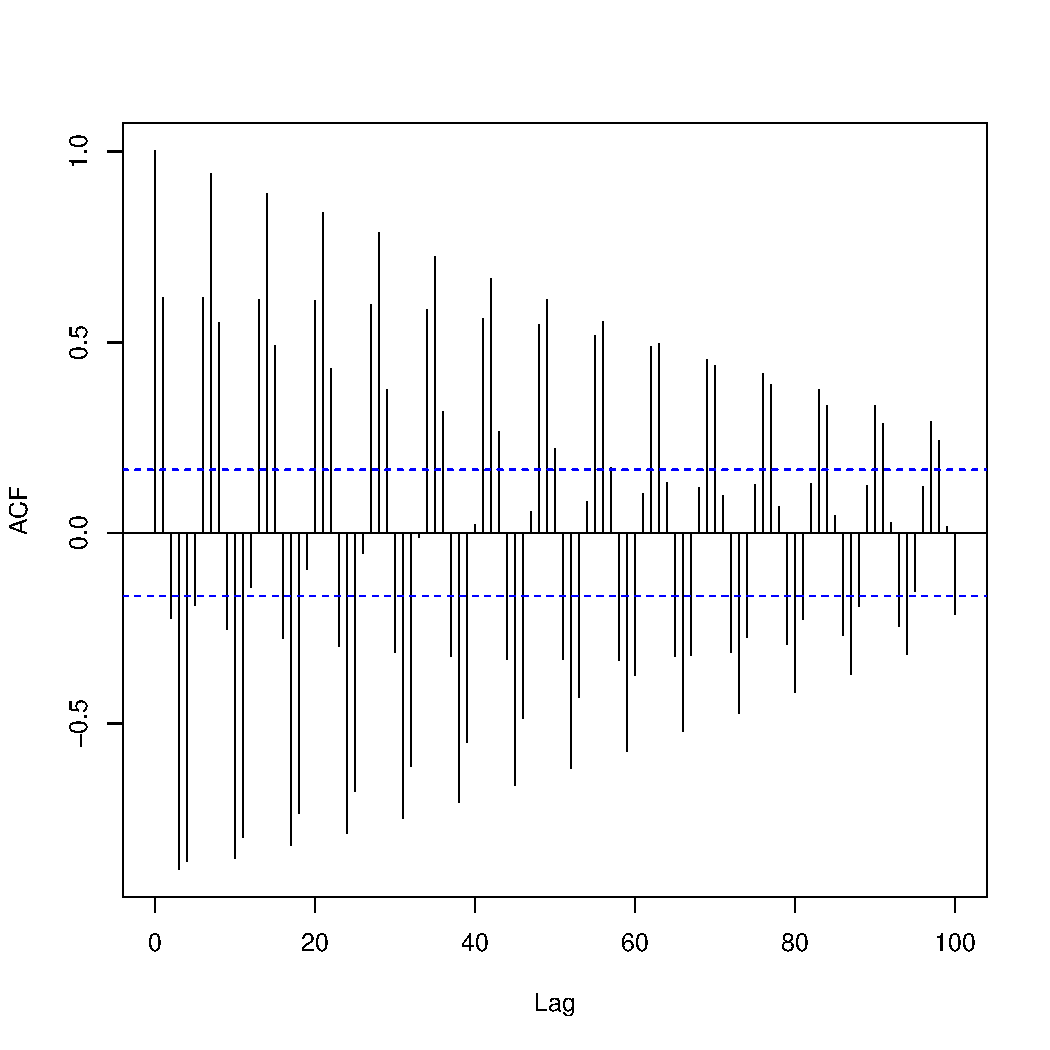
\includegraphics{img/acf-sine.pdf}}
            \caption{Autocorrelation function of sine function.}
            \label{img:period-acf}
        \end{center}
    \end{figure}

    The algorithm for automatic period identification is demonstrated in Algorithm \ref{alg:period-find}.
    It looks for periodically repeated significant values of ACF function. At some rate these values have to
    be decreased to zero. In the infinity ACF function converges to zero.

    The algorithm as input takes only time series. If there is a unit root present, then differencing is applied.
    Calculation of autocorrelation function of input time series follows and finding the index of its highest
    value. Then it checks if there are significant values of ACF present at following $n*period$ indices.
    There have to be present at lease two consecutive values of ACF, so $n$ takes values from $1,2,3\dots$

    \begin{algorithm}
        \caption{Find period of time series} \label{alg:period-find}
        \begin{algorithmic}[1]
        \Function{findFrequency}{$int[] ts$}
            \If{$unitRootPresent(ts)$} \Comment{e.g. ADF test}
                \State $ts \gets diff(ts)$ \Comment{first order differences}
            \EndIf
            \State $acf \gets acf(ts)$ \\
                        \Comment{returns index of the highest value}
            \State $period \gets findHighest(ts, period)$
            \While{$period * 2 < ts.length$}
                \If{$checkPeriodExists(x, ts)$}
                    \State \Return $period$
                \EndIf
              \State $period \gets findHighest(ts, period)$
            \EndWhile
            \State \Return $1$
        \EndFunction
        \end{algorithmic}
    \end{algorithm}

%%%%%%%%%%%%%%%%%%%%%%%%%%%%%%%%%%%%%%%%%%%%%%%%%%%%%%%%%%%%%%%%%%%
\chapter{Analytical Forecasting Process} \label{chap:models-demonstration}
In the previous chapter several time series models were described. However, in Hawkular only few of them were
selected and implemented.

This chapter demonstrates targeted models on real time series. There is also conducted a
statistical comparison of the models. This chapter also contains theory how different models should be compared. At
the end there is a discussion which models were selected for usage in Hawkular.

    %%%%%%%%
    \section{Evaluating Forecasting Accuracy} \label{sec:mse-mae}
    In order to evaluate a forecasts produced by particular model it is important to calculate the errors of the
    forecasts. There are several statistics for evaluating forecasting accuracy. The most used ones are mean squared
    error (MSE) \ref{eq:accuracy-mse} and mean absolute error (MAE) \ref{eq:accuracy-mae} \cite{statistika}. The
    difference between them is that MSE emphasizes the extremes while MAE is more robust to outliers
    \cite{hyndman-forecasting}.

    \begin{gather} \label{eq:accuracy-mse}
         MSE = \frac{1}{n} \sum_{i=1}^{n}(y_i - \hat{y_i}) \\
         MAE = \frac{1}{n} \sum_{i=1}^{n} \abs{y_i - \hat{y_i}} \label{eq:accuracy-mae}
    \end{gather}

    %%%%%%%%
    \section{Measuring Model Quality} \label{sec:model-quality}
    When comparing multiple models, statistics like MSE or MAE are not the best objective functions. Comparison
    based on this statistics can select complicated model with lots of parameters, which may overfit training data
    and most importantly it selects less robust model \cite{cipra}. Therefore for comparison multiple models another
    factors have to be added to the objective function. These factors are number of parameters of the model.

    The most used criteria for model sections are: Akaike information criterion (AIC) and Bayesian information
    criterion (BIC). Model with lower information criterion is preferred.

    \begin{gather} \label{eq:aic}
        AIC = 2 k - \ln(L) \\ \nonumber
        BIC = k \ln(n) - 2 \ln(L)
    \end{gather}

    Equations for AIC and BIC are listed in \ref{eq:aic}. Number of parameters of the model is represented by $k$.
    Number of observations is denoted by $n$ and $L$ stands for maximized value of the likelihood function of the
    model. In case for exponential smoothing it is minimized sum of squared error of one step ahead prediction of
    training data set.

    From the equations it can be seen that BIC penalizes models with more parameters. There is also AIC criterion with
    correction form \ref{eq:aicc}. Corrected version of AIC more penalizes longer models.

    \begin{eqnarray} \label{eq:aicc}
        AICc = AIC + \frac{2k(k+1)}{n-k-1}
    \end{eqnarray}

    %%%%%%%%
    \section{Models Demonstration} \label{sec:models-demonstration}
    An analytical process of modelling time series starts with plotting the data and fitting various models chosen by
    forecaster's previous experience. In second step forecaster compares statistics of those models and chooses the one
    that describes data the best.

    In this section real time series is modelled using time series models discussed in Chapter \ref{chap:models}.
    Chosen time series is \emph{austourists} from R package \texttt{fpp}. This series is a measurement of quarterly
    visitor nights spent by international tourists in Australia. It was chosen on purpose because it contains trend
    and seasonality.

    On the first Chart \ref{img:simple-models} there is depicted na\"{i}ve, average and drift model. Average model is
    just an overall average of the whole time series. It does not change over time. However there could be an online
    version of this algorithm for which an average would be calculated for each new value.

    Na\"{i}ve and drift model copy values of time series with lag of one observation. These two models differs in
    forecasts where drift model is capable of forecasting trends.

    \begin{figure}[H]
        \begin{center}
%            \resizebox{12cm}{8cm}{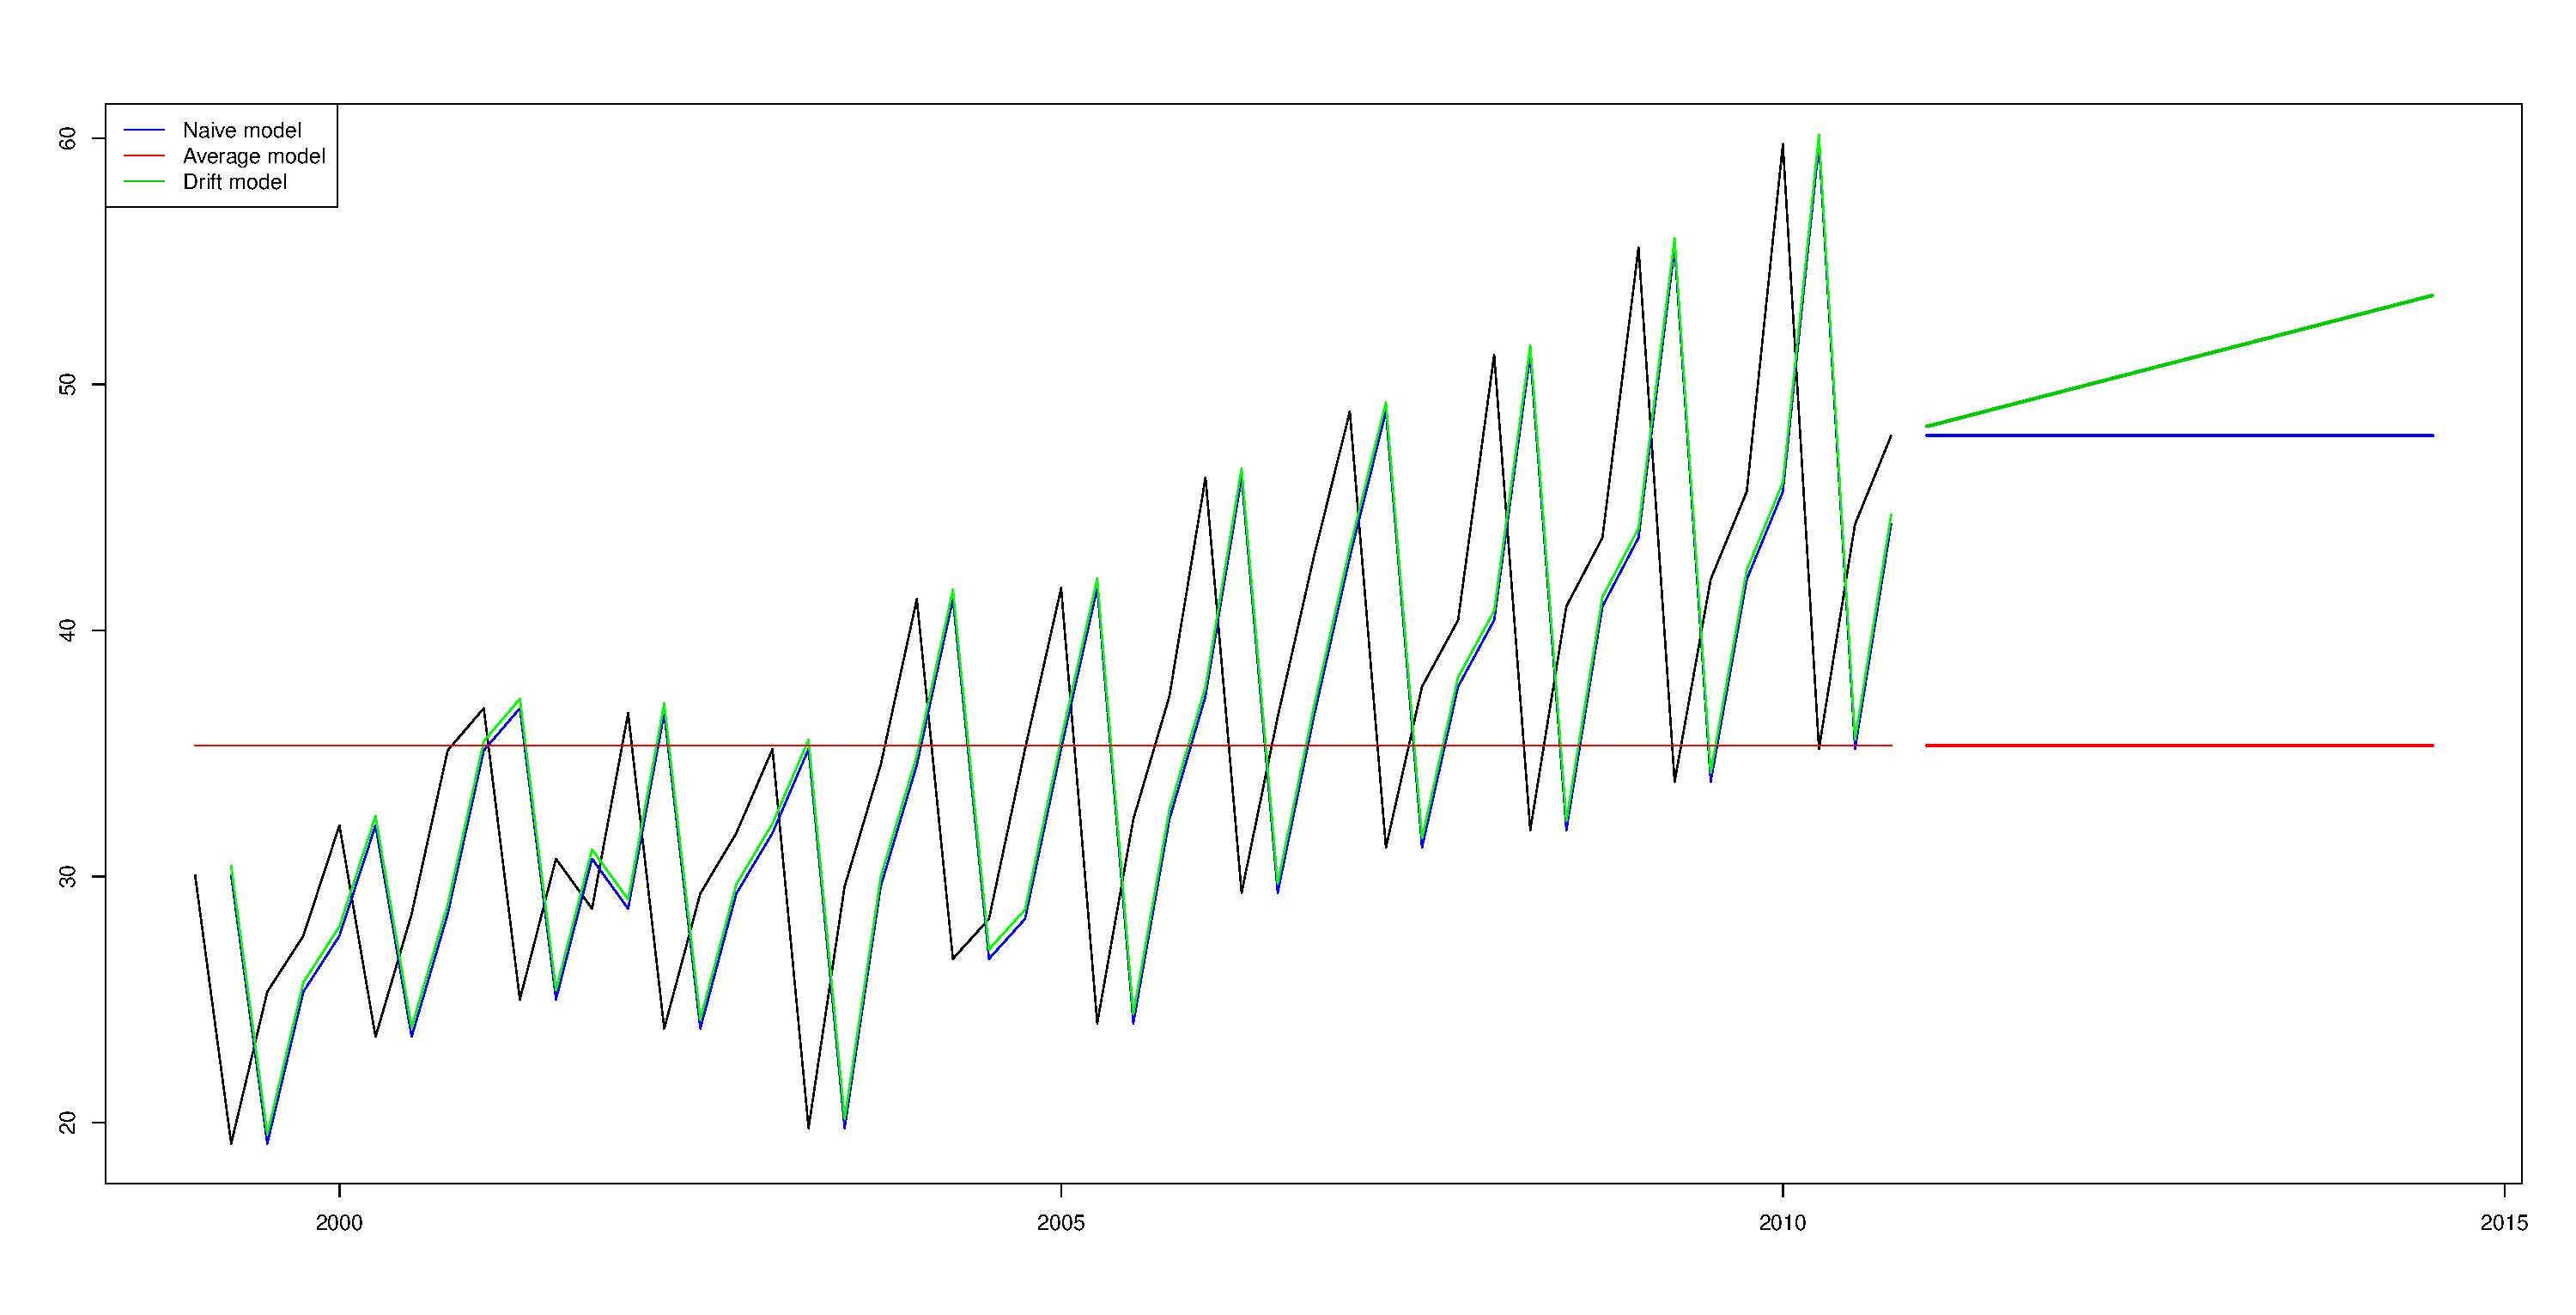
\includegraphics{img/simple-models.pdf}}
            \scalebox{0.255}[0.4]{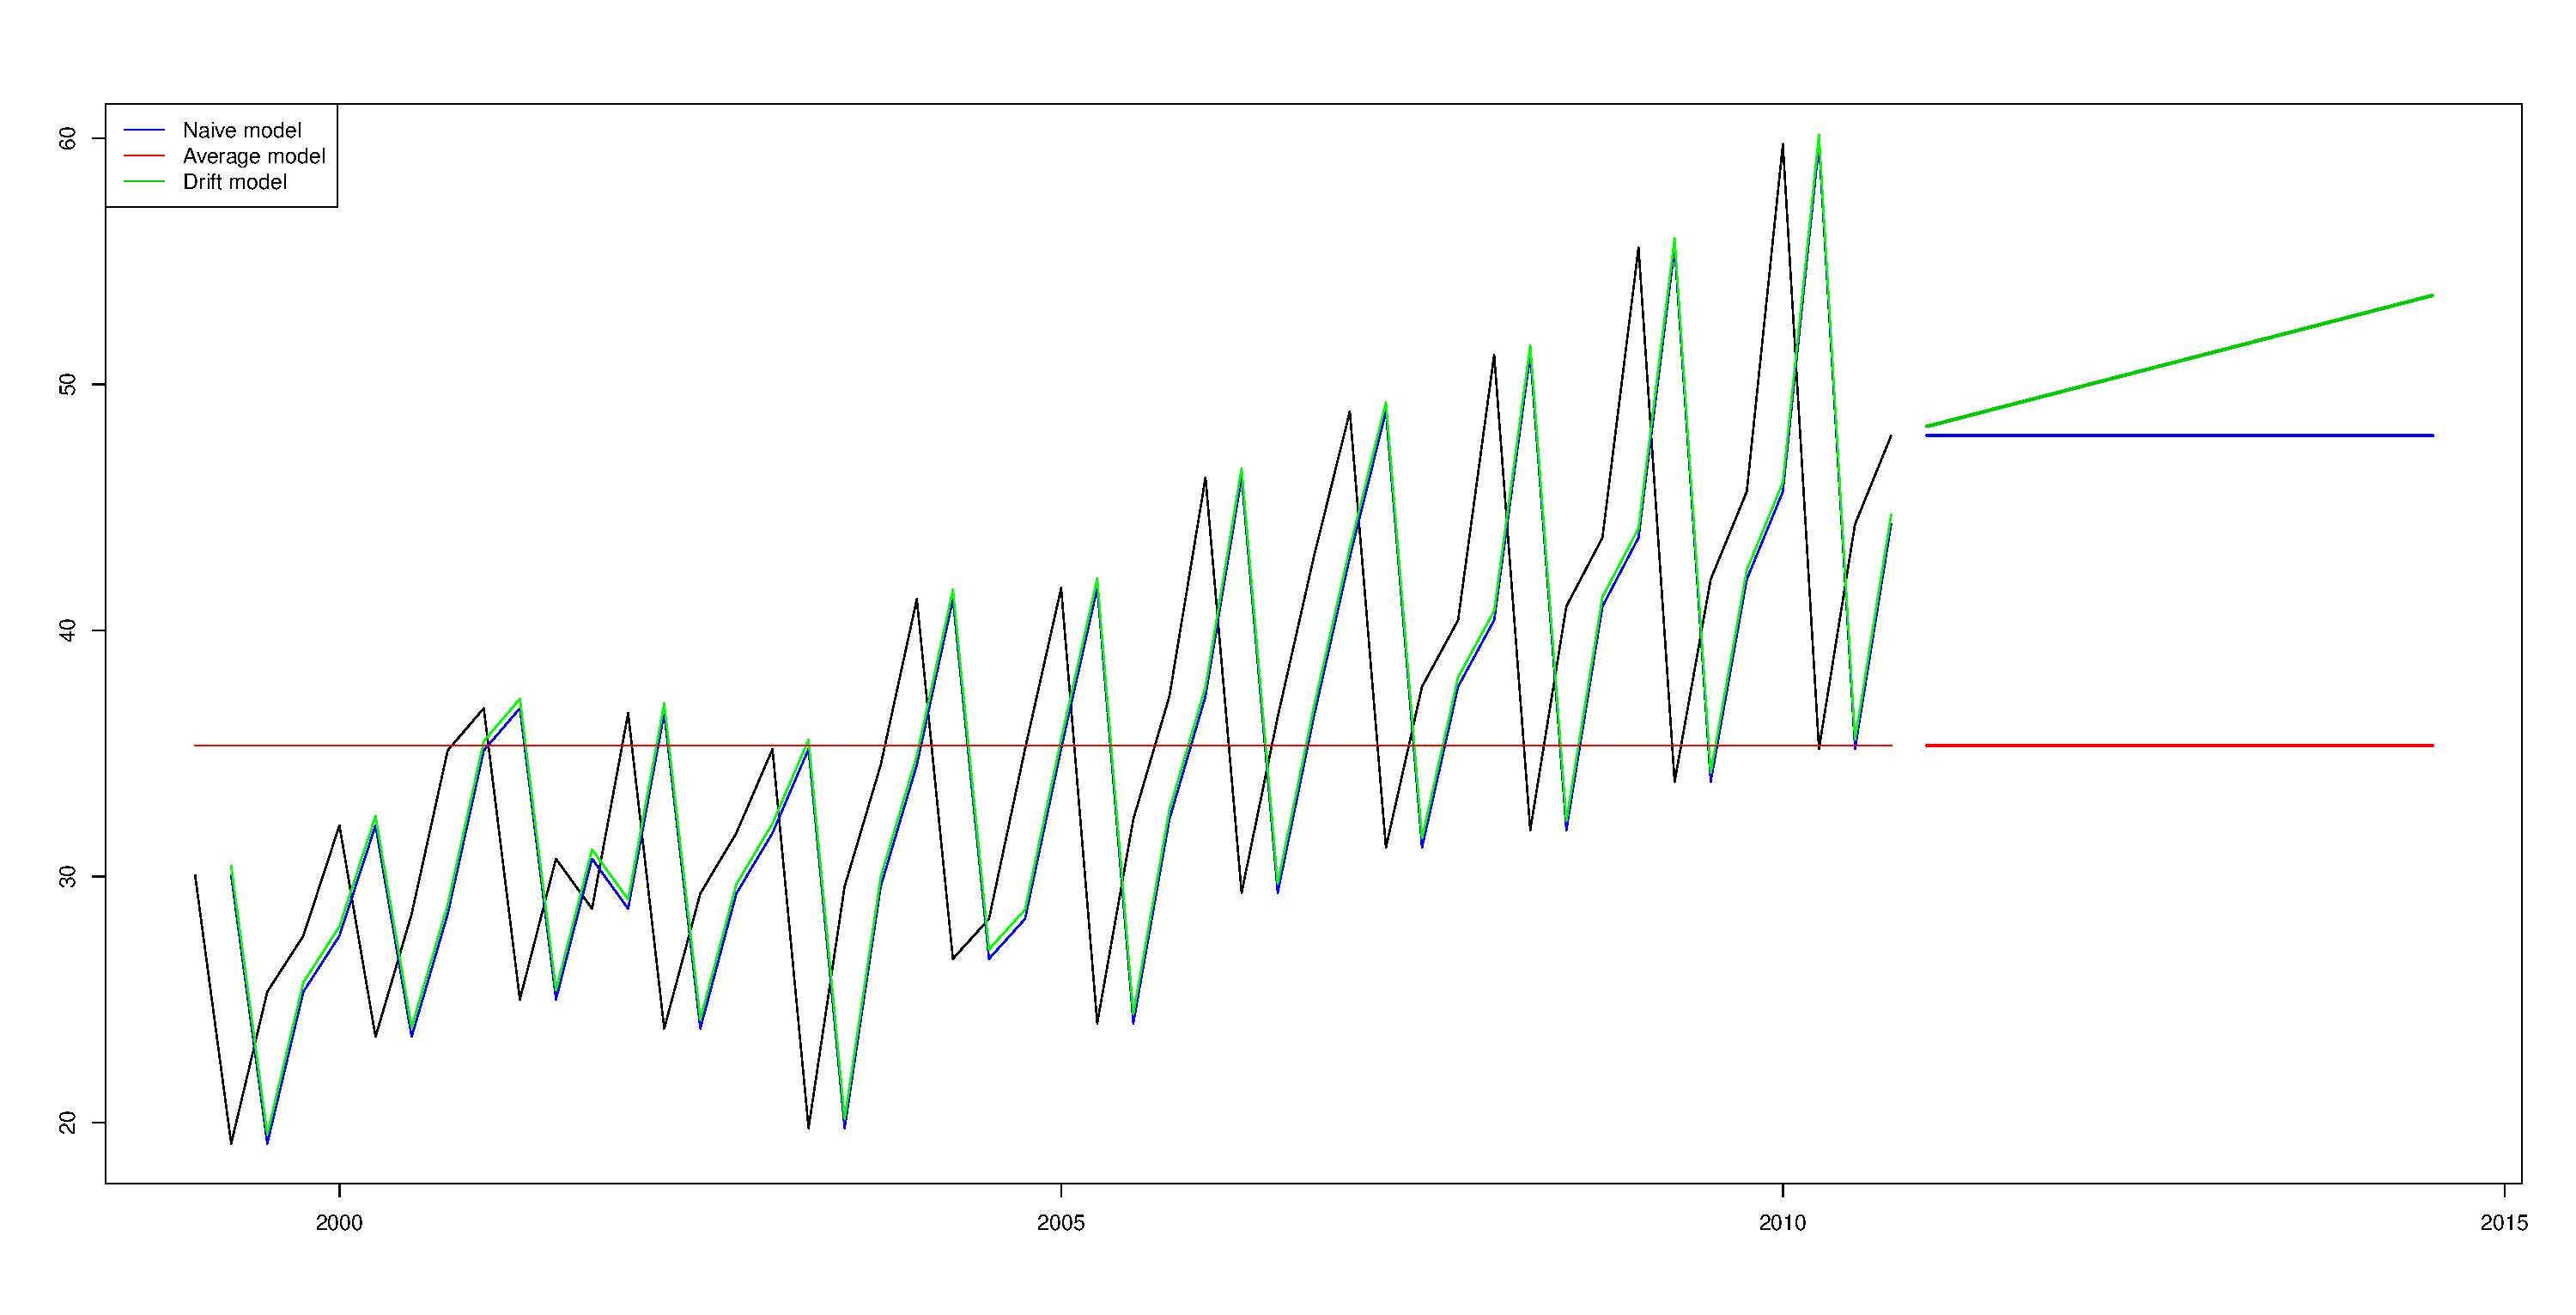
\includegraphics{img/simple-models.pdf}}
            \caption{Simple models on \emph{austourists}.}
            \label{img:simple-models}
        \end{center}
    \end{figure}

    Exponential smoothing models are depicted in Chart \ref{img:exp-smoothings}. For this particular series it is
    obvious that seasonal model is the best describing modelled time series.

    In the beginning it can be seen how is the seasonal model changing and learning the seasonal pattern from data.
    Learning and adaptivity to new trends depends on smoothing parameters of the models. Higher values of parameters
    allows the model quicker adapt to changes. Models with lower smoothing parameters are more robust to the changes.

    \begin{figure}[H]
        \begin{center}
            \scalebox{0.255}[0.27]{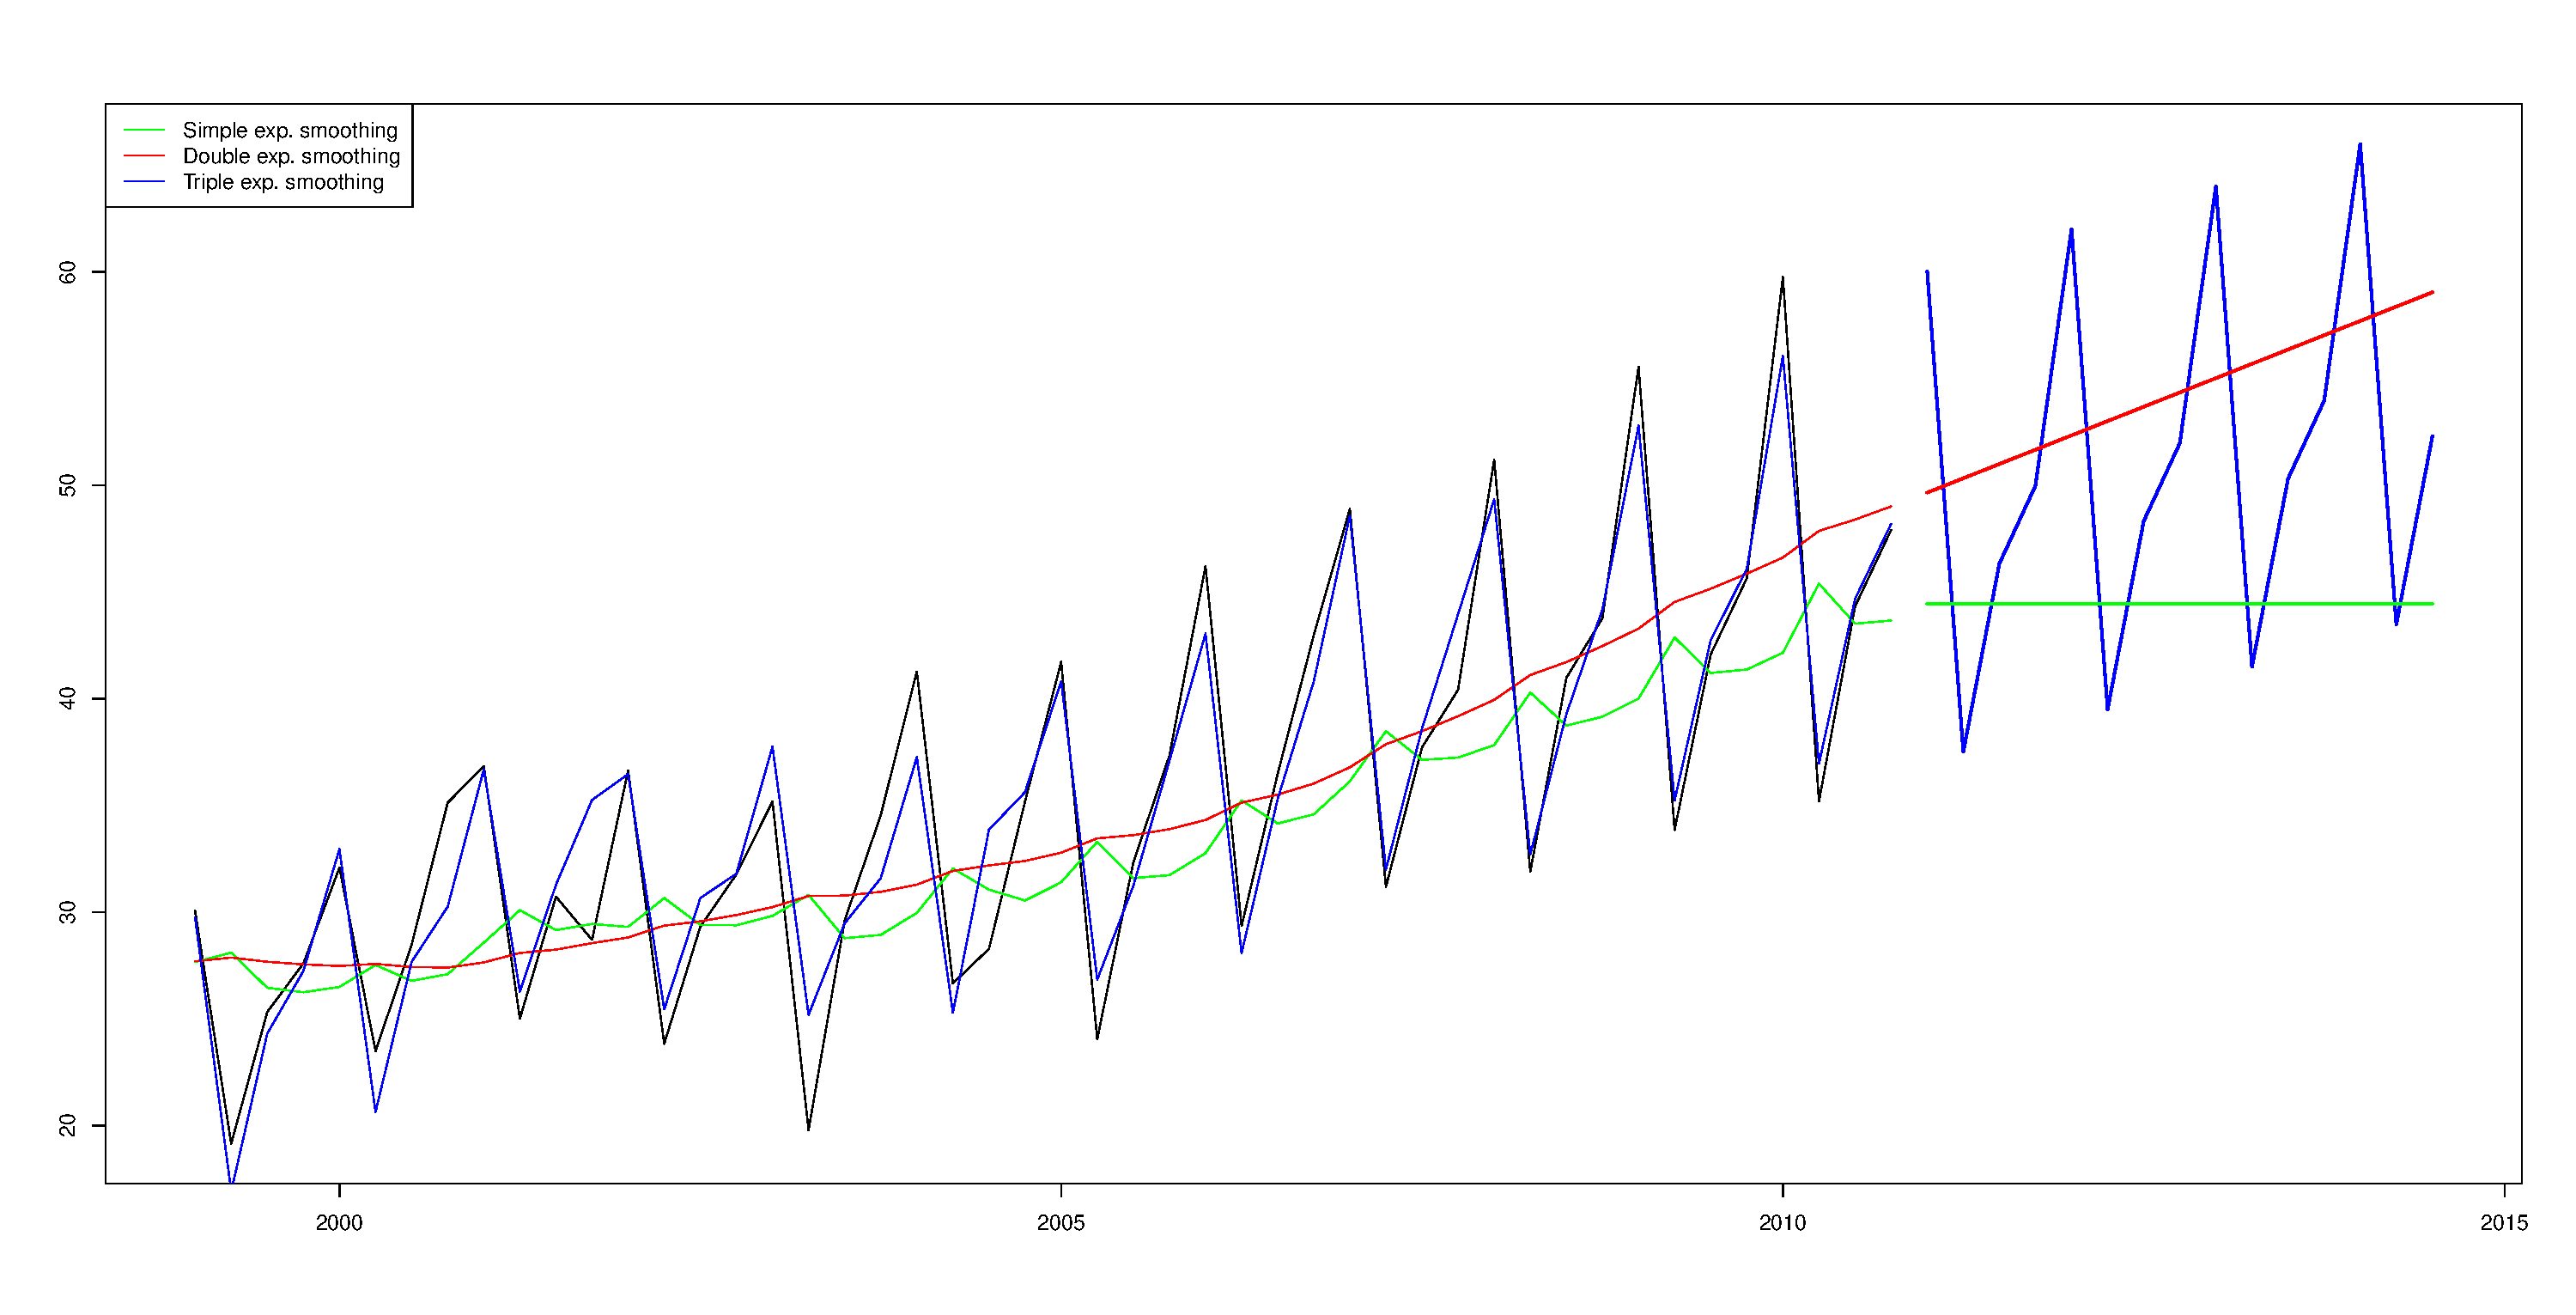
\includegraphics{img/exp-smoothings.pdf}}
            \caption{Exponential smoothing models on \emph{austourists}.}
            \label{img:exp-smoothings}
        \end{center}
    \end{figure}

    \begin{figure}[H]
        \begin{center}
            \scalebox{0.255}[0.27]{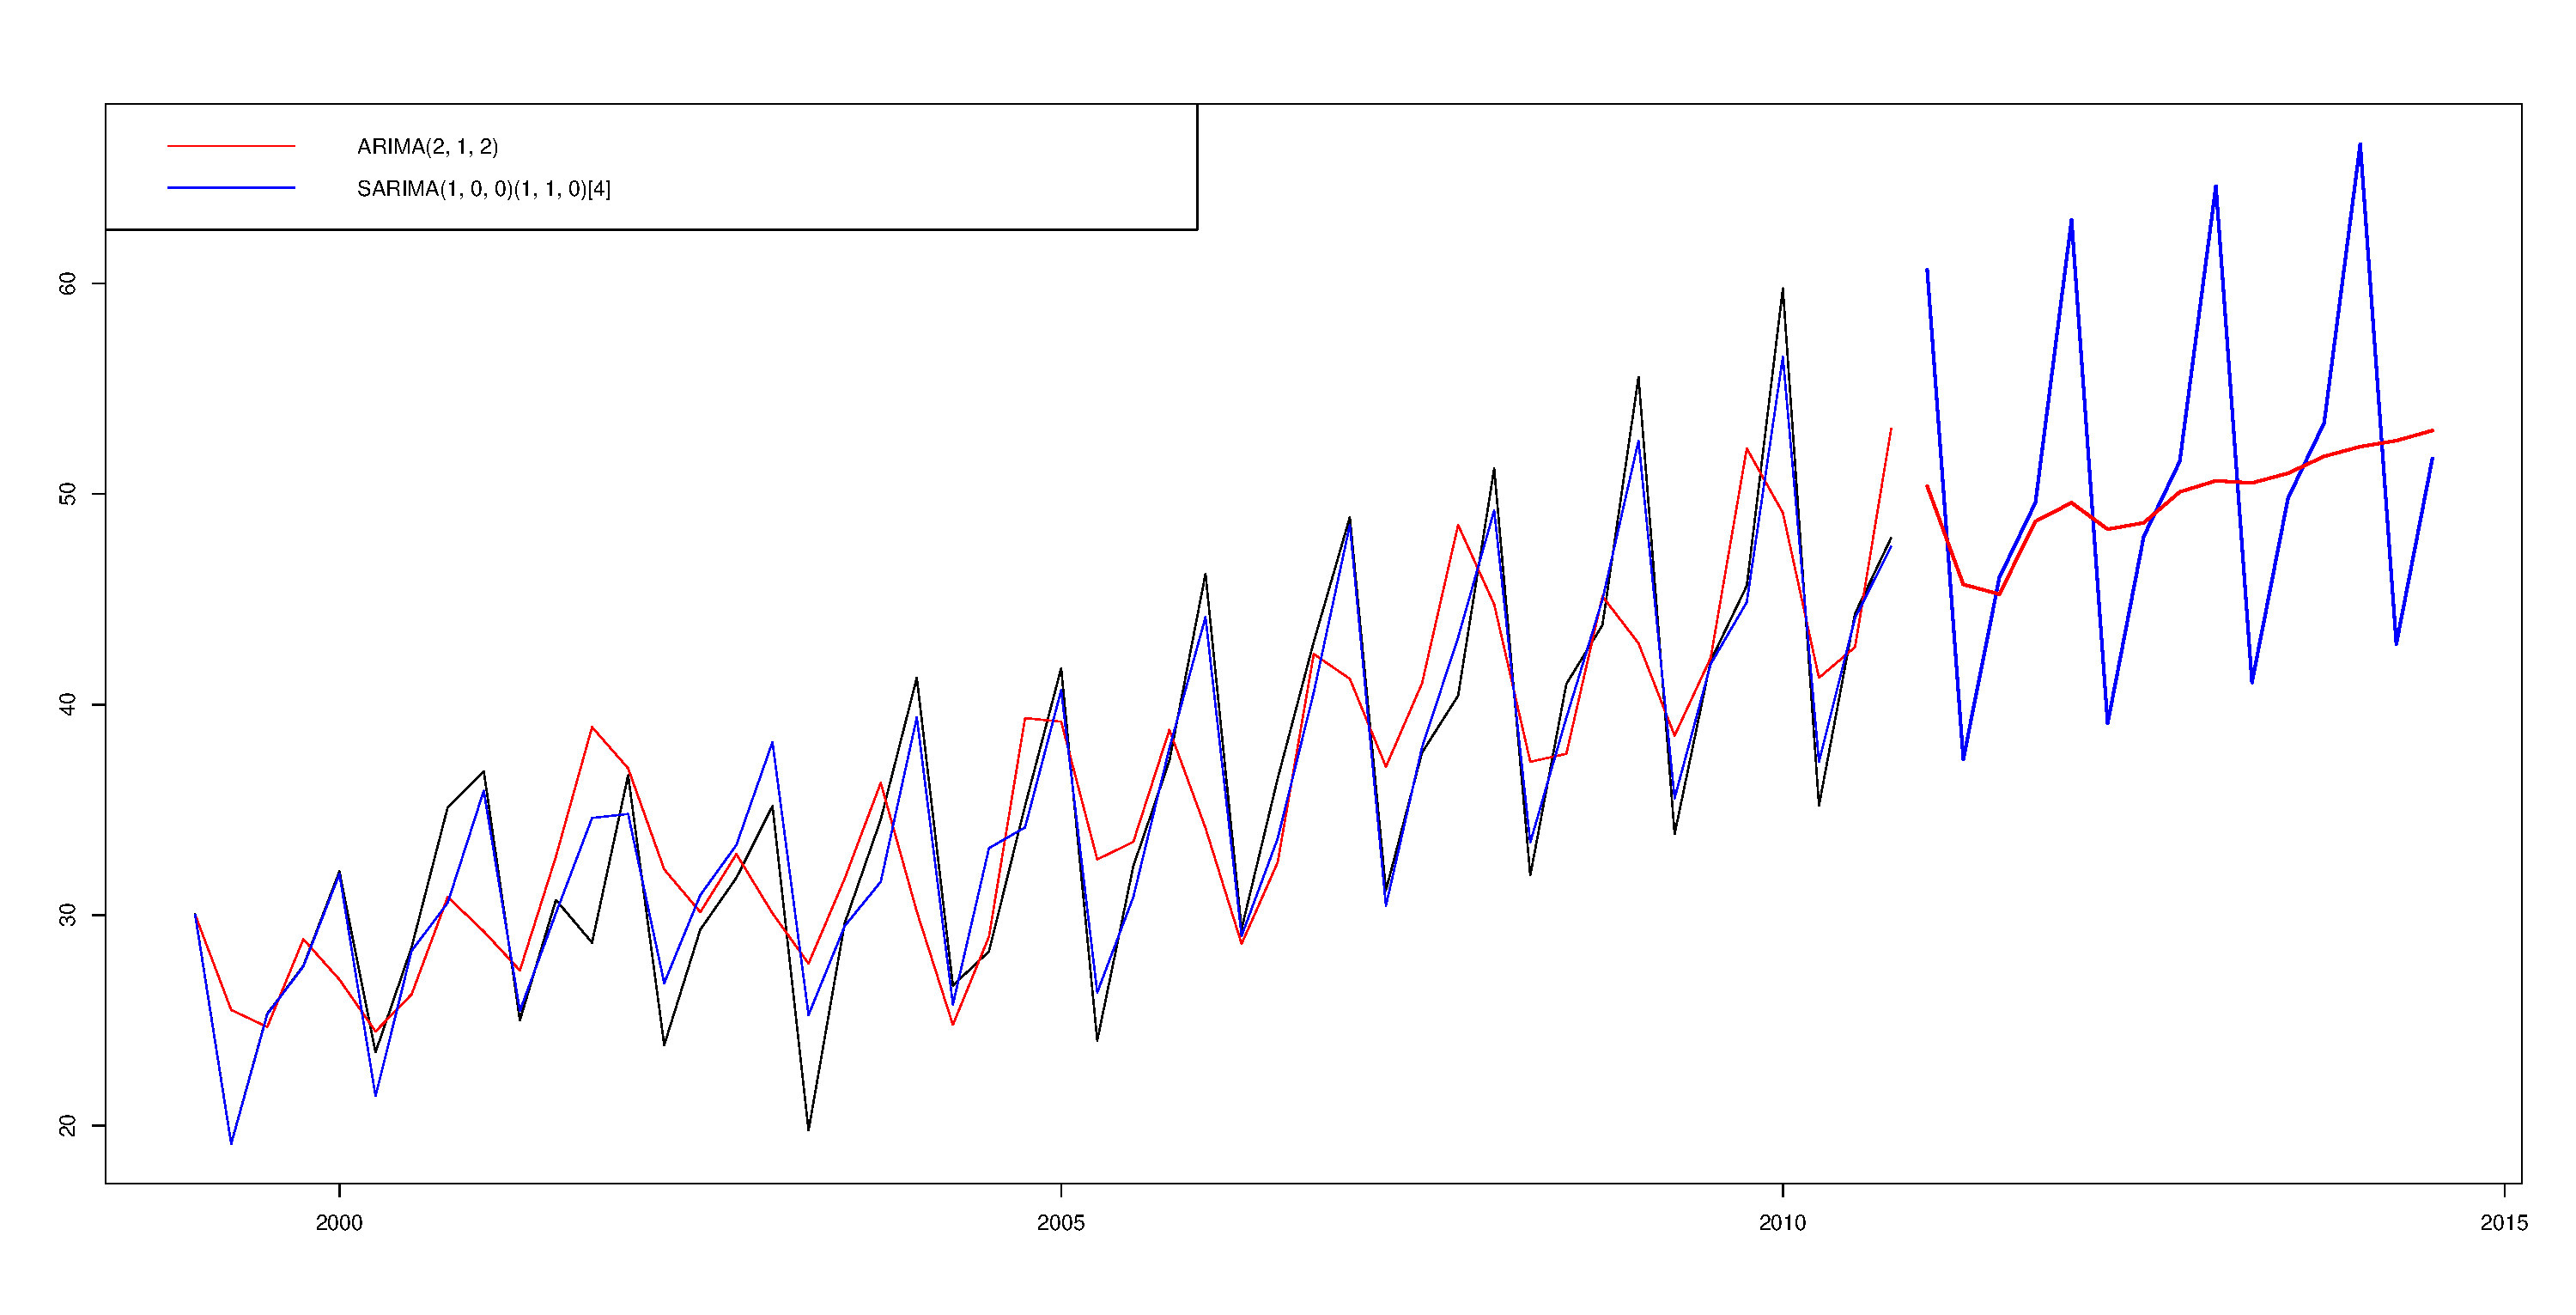
\includegraphics{img/arima-sarima.pdf}}
            \caption{Arima models on \emph{austourists}.}
            \label{img:arimas}
        \end{center}
    \end{figure}

    ARIMA models are shown in Chart \ref{img:arimas}. Non-seasonal model is already capable of capturing some seasonal
    patterns but it is more random whereas seasonal patterns should be of fixed period. Therefore seasonal ARIMA with
    dedicated model for each period is more appropriate.

    \begin{table}[h]
        \begin{center}
            \begin{tabular}{l|r|r|c}
                    \textbf{Model} & \textbf{MSE} & \textbf{MAE} & \textbf{AIC} \\ \hline \hline
                    Na\"{i}ve & 104.74 & 8.64 & \\
                    Drift & 104.60 & 8.47 & \\
                    Average & 79.91 & 7.14 & \\ \hline
                    Simple exp. smoothing & 53.54 & 5.91 & 380.88 \\
                    Double exp. smoothing & 44.41 & 5.28 & 375.90 \\
                    Triple exp. smoothing & 5.34 & 1.71 & 282.73 \\ \hline
                    Linear regression & 41.85 & 5.10 & 321.46 \\ \hline
                    ARIMA(2, 1, 2) & 30.88 & 4.35 & 310.6 \\
                    SARIMA(1, 0, 0)(1, 1, 0)[4] & 4.79 & 1.63 & 206.95 \\
            \end{tabular}
            \caption{Statistics of models.}
            \label{tab:models-stat}
        \end{center}
    \end{table}

    Statistics produced by each model are listed in Table \ref{tab:models-stat}. Models with the lowest one
    step ahead prediction error are seasonal ARIMA and triple exponential smoothing which is correct for this highly
    seasonal time series.

    As it was discussed in Section \ref{sec:model-quality} AIC criterion should be used for models comparison. From
    Table \ref{tab:models-stat} it can be seen that AIC and MSE are related, however MSE of double exponential smoothing
    is $8.3$ times higher than MSE of triple exponential smoothing, whereas AIC of double exponential smoothing is
    only $1.3$ times higher. From this example it is obvious how AIC discriminates models with more parameters.

%%%%%%%%%%%%%%%%%%%%%%%%%%%%%%%%%%%%%%%%%%%%%%%%%%%%%%%%%%%%%%%%%%%
\chapter{Existing Solutions}
Before going directly to the design and implementation let's briefly look at existing monitoring solutions and libraries
for time series modelling.

In the next section not only direct competitors of Hawkular are described but also
generally available software of this kind. Because Hawkular is still only an upstream project and not deliverable
product for the customers, thereby Jboss Operations Network (JON) is considered as its alternative.

However, this work does not focus on precise comparison of monitoring applications. It is only mentioned for wider
overview of this domain.

    %%%%%%%%
    \section{Monitoring and Management Applications}
    There are many monitoring solutions available out there. Some of them are offered as service (SaaS) and other need
    to be deployed in customer's environment.

    The most important features for each application are highlighted altogether with information how it differs from its
    competitors and if application offers predictive capabilities.

        %%%%%%%%
        \subsection{New Relic}
        New Relic was the first monitoring solution offered as SaaS \cite{new-relic}. It focuses on application
        performance rather than infrastructure view.

        Monitoring of Java applications is done by agents. Because agent manipulates with bytecode it is able to
        identify business transactions and monitor for instance utilization of REST endpoints.

        Agents also automatically discover databases connected to the application being monitored. From alert
        prediction perspective New Relic does not offer any alert prediction or predictive charts.

        %%%%%%%%
        \subsection{Dynatrace Ruxit}
        Ruxit is another popular SaaS solution for monitoring middleware applications. Monitoring is also done by agents
        which instrument bytecode so the application is also able to monitor business transactions. Ruxit differs from
        others in offering root cause analysis rather than firing multiple alerts \cite{ruxit}. It directly shows
        causing problems with visual representation. Ruxit does not offer any predictive alerting or charts.

        %%%%%%%%
        \subsection{Open Source Projects}
        As Hawkular is an open source project it is important to mention its direct competitors from this area.
        There are two major open source projects. The first one is Nagios and second Zabbix. Nagios was started in
        1991 and Zabbix in 2001 therefore both are more than fifteen years old.

        In comparison to Hawkular, Ruxit or New Relic the user interface of these two projects feels much older.
        At the time of writing this thesis last contribution to Nagios was from 17th September 2015 and Nagios
        project was active until the last moment. Both of these projects do not offer alert prediction.

        %%%%%%%%
        \subsection{HP OpenView and IBM Tivoli}
        The biggest monitoring solutions offered by these two software giants are HP OpenView and IBM Tivoli. Both are
        composed of many independent products. Solution from HP does not offer any predictive capabilities.

        Operations Analytics, one of IBM Tivoli products can automatically detect correlations between
        metrics which can lead to detection of application issues, for example an anomaly detection
        \cite{tivoli-predictive-insights}.

        Another part of Tivoli solution\,--\,Netcool Network Management is capable
        of predicting events. There is also another predictive analysis in Tivoli Monitoring
        module\footnote{Available at
        \url{https://www.ibm.com/developerworks/community/wikis/home?lang=en\#/wiki/Tivoli+Monitoring/}.}.
        In the online document there it is mentioned that predictive engine does not work on real time streams of data.
        Tivoli is definitely a big solution and in order to get real predictive capabilities it would require to
        contact IBM support.

    %%%%%%%%
    \section{Libraries For Time Series Forecasting} \label{sec:libraries-for-ts}
    In Java there is only one publicly available library for time series modelling. The library is called
    OpenForecast\footnote{Available at \url{http://www.stevengould.org/software/openforecast/index.shtml}.}. It contains
    models like na\"{i}ve, linear regression and exponential smoothing models. Whereas the library is open source, code
    was reviewed and tested. Some assumptions about the implementation were made. The parameters of some models are
    not estimated correctly. For example in linear regression slope and intercept are not estimated by minimizing
    sum of squared errors.

    The library provides nice feature called automatic forecaster which selects the best model for given
    time series, however the code produces null pointer exception. The bug was identified but the library is not
    maintained anymore.

    The performance of the library was also tested. Table \ref{tab:open-forecast-perf} contains execution times of
    optimizers for simple, double and triple exponential smoothing models. The tested time series is generated sine
    function of length 200 observations. The result is compared against execution times of R's function \texttt{ets}
    from \texttt{forecast} package.

    \begin{table}[h]
        \begin{center}
            \begin{tabular}{l|c|c}
                \textbf{Model} & \textbf{OpenForecast} & \textbf{R \texttt{forecast}} \\ \hline \hline
                Simple ex. & 4.91 sec. & 0.003 sec.\\
                Double ex. & 9.31 sec. & 0.006 sec.\\
                Triple ex. & 6.45 sec. & 0.209 sec.\\
            \end{tabular}
            \caption{Execution time of parameters estimation for exponential smoothing models.}
            \label{tab:open-forecast-perf}
        \end{center}
    \end{table}

    From the table it is obvious that R's implementation is much faster. For example optimization of thousand double
    exponential smoothing models would take about two and half hours. This results are not acceptable for Hawkular in
    real time environment.

    Another possibility is to directly use R implementation. There are various libraries\footnote{The most widely used:
    RCaller and JRI.} which allow executing R code from Java, however it requires installed R system in the target
    environment.

    Other possible solution is to use Rengin\footnote{Available at \url{http://www.renjin.org/}}\,--\,JVM interpreter
    for R. However \texttt{forecast} package depends on other package which invocates native C++ code for optimized
    computations. Therefore \texttt{forecast} package can not be used with Rengin.
